\documentclass[12pt]{article}
\usepackage[english]{babel}
\usepackage[letterpaper,margin=1in]{geometry}
\usepackage[parfill]{parskip}
\usepackage{graphicx}
\usepackage{mathtools}
\usepackage{amssymb}
\graphicspath{{img/}}
\usepackage{hyperref}
\frenchspacing
\author{Ariel Davis (azdavis), Jerry Yu (jerryy)}
\date{\today}
\title{15-418 Final Project Report}
\begin{document}
\maketitle

\section{Overview}

We implemented portrait mode in parallel.
Portrait mode has traditionally been done by high end DSLR camera hardware,
which the foreground of the subject is in focus and the background is blurred.
We have chosen to use a software-only image processing approach to this problem,
segmenting the image into the foreground and blurring the background.

On our largest images, we were able to achieve 150x speedup with CUDA on GPUs
and 11x speedup with OpenMP on CPUs.

\begin{figure}[!htb]
    \begin{minipage}{0.48\textwidth}
        \centering
        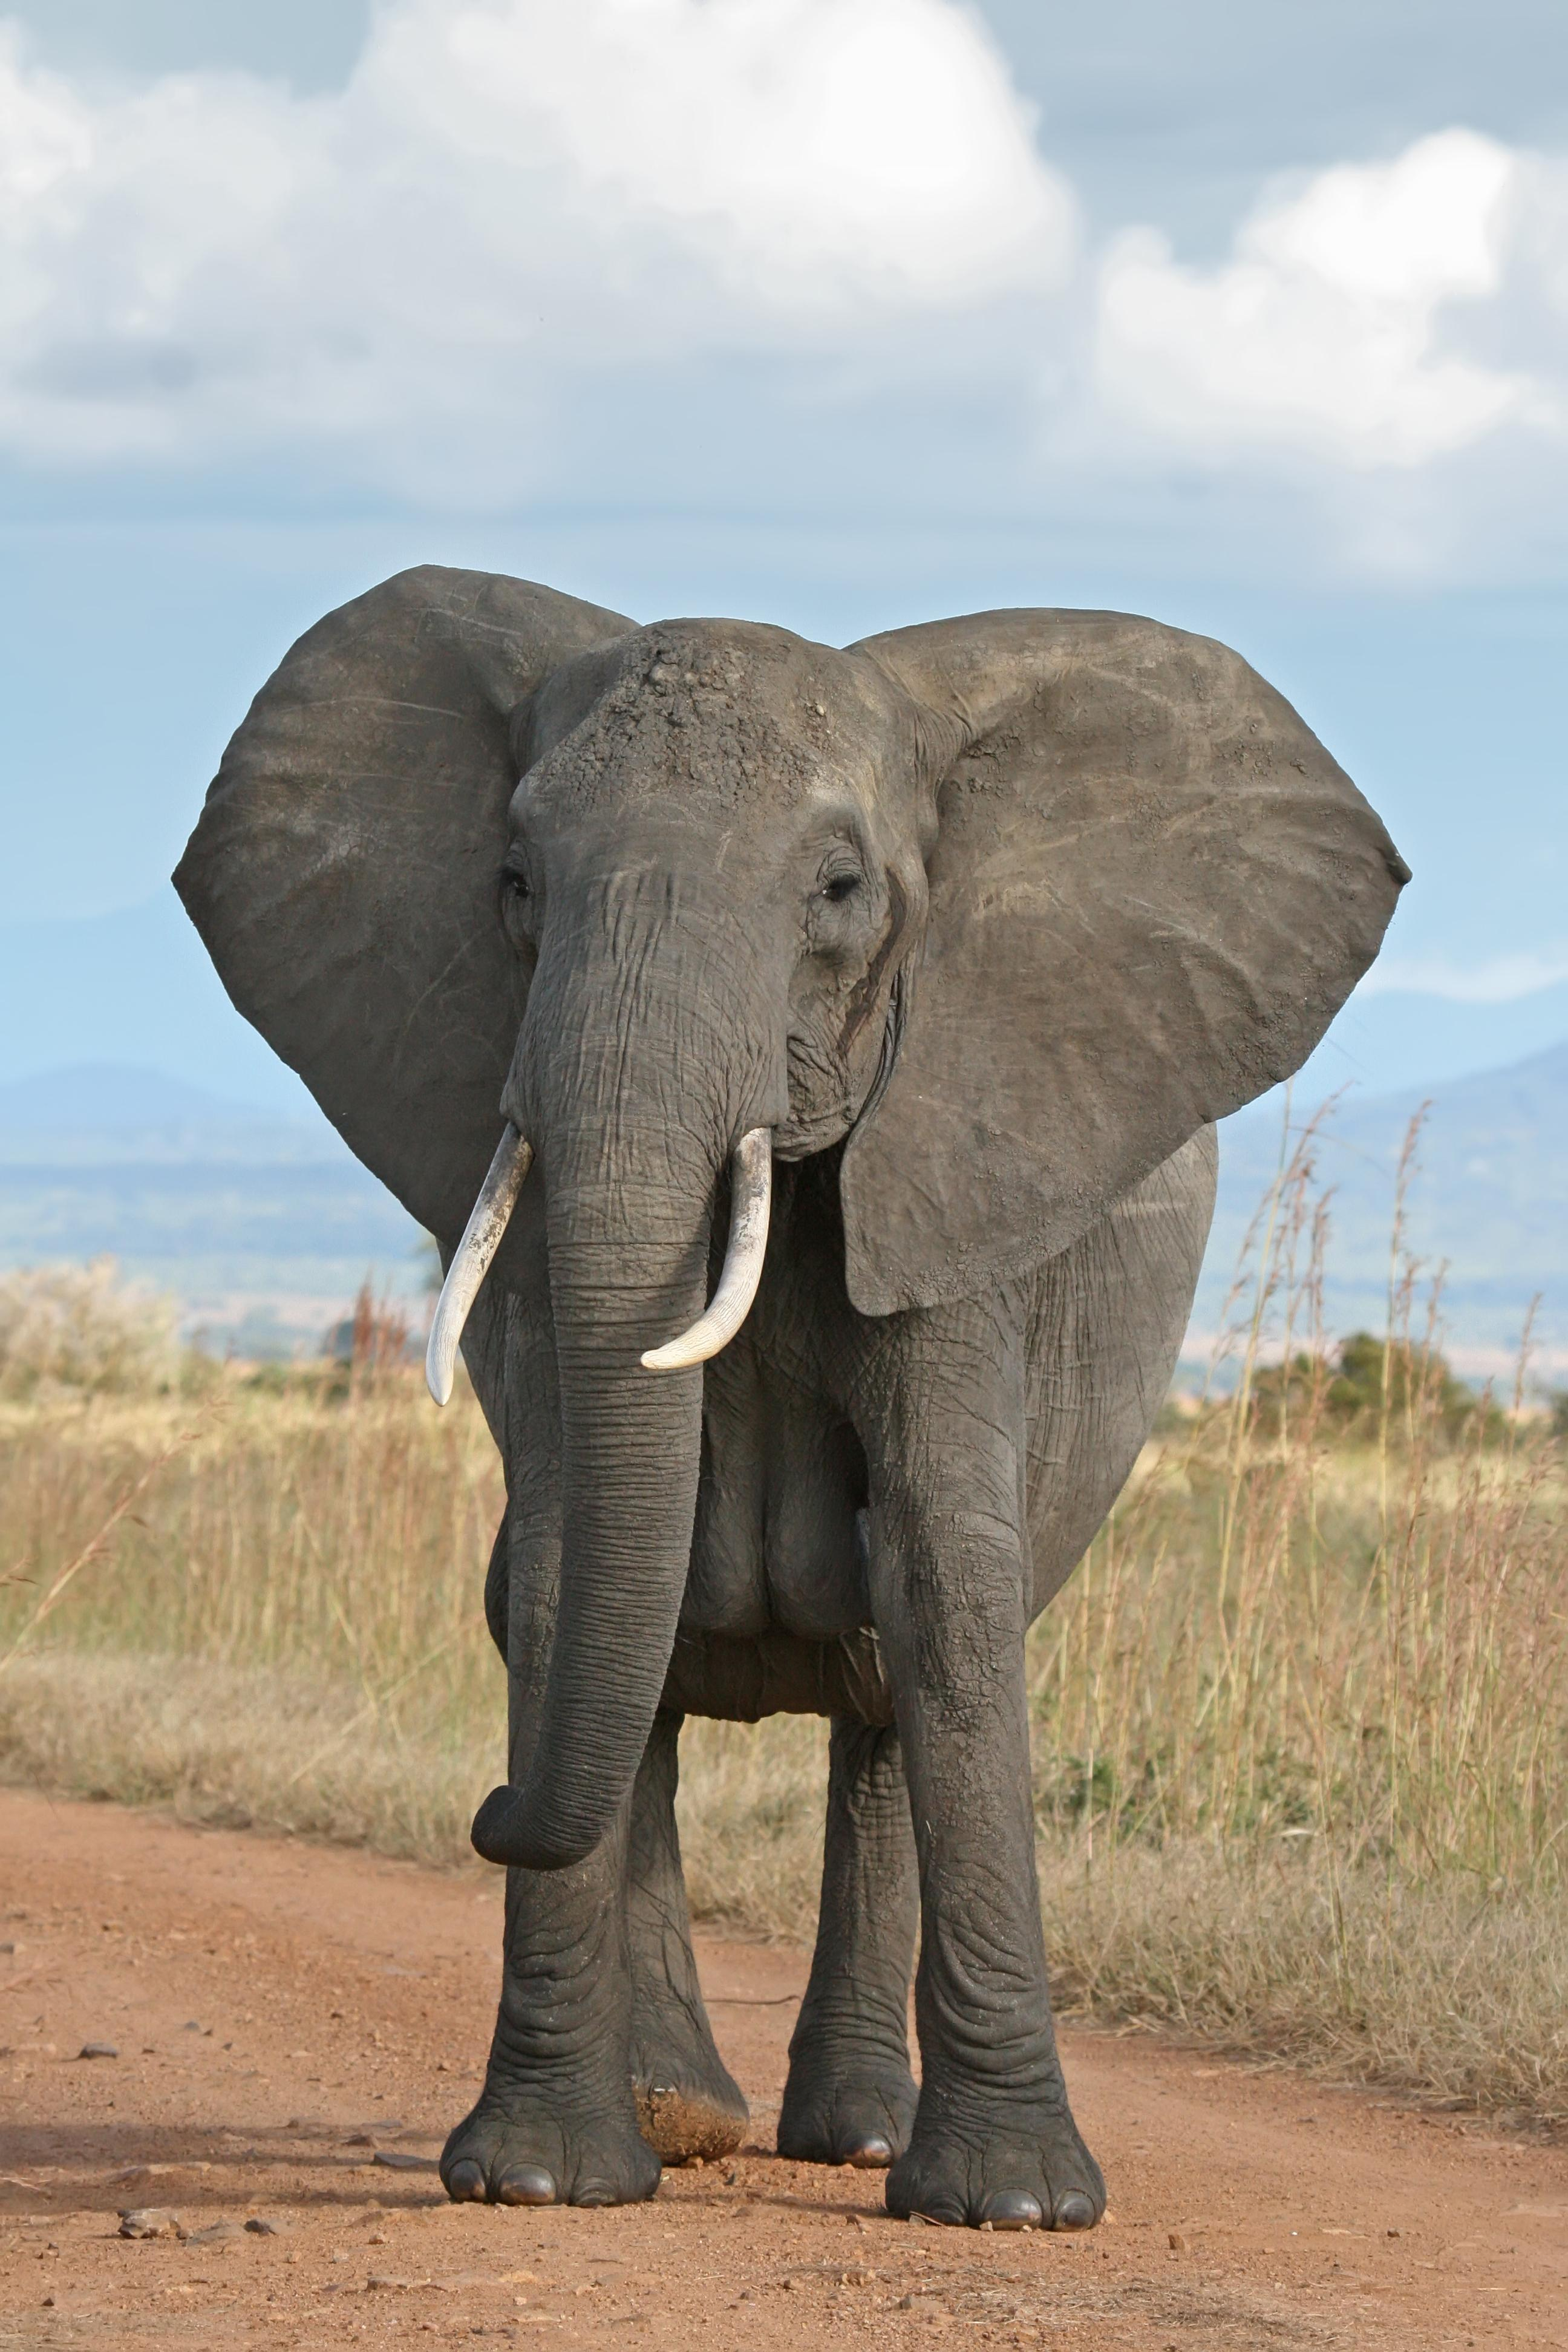
\includegraphics[width=0.9\linewidth]{large_elephant.jpg}
        \caption{Input Image}
    \end{minipage}\hfill
    \begin{minipage}{0.48\textwidth}
        \centering
        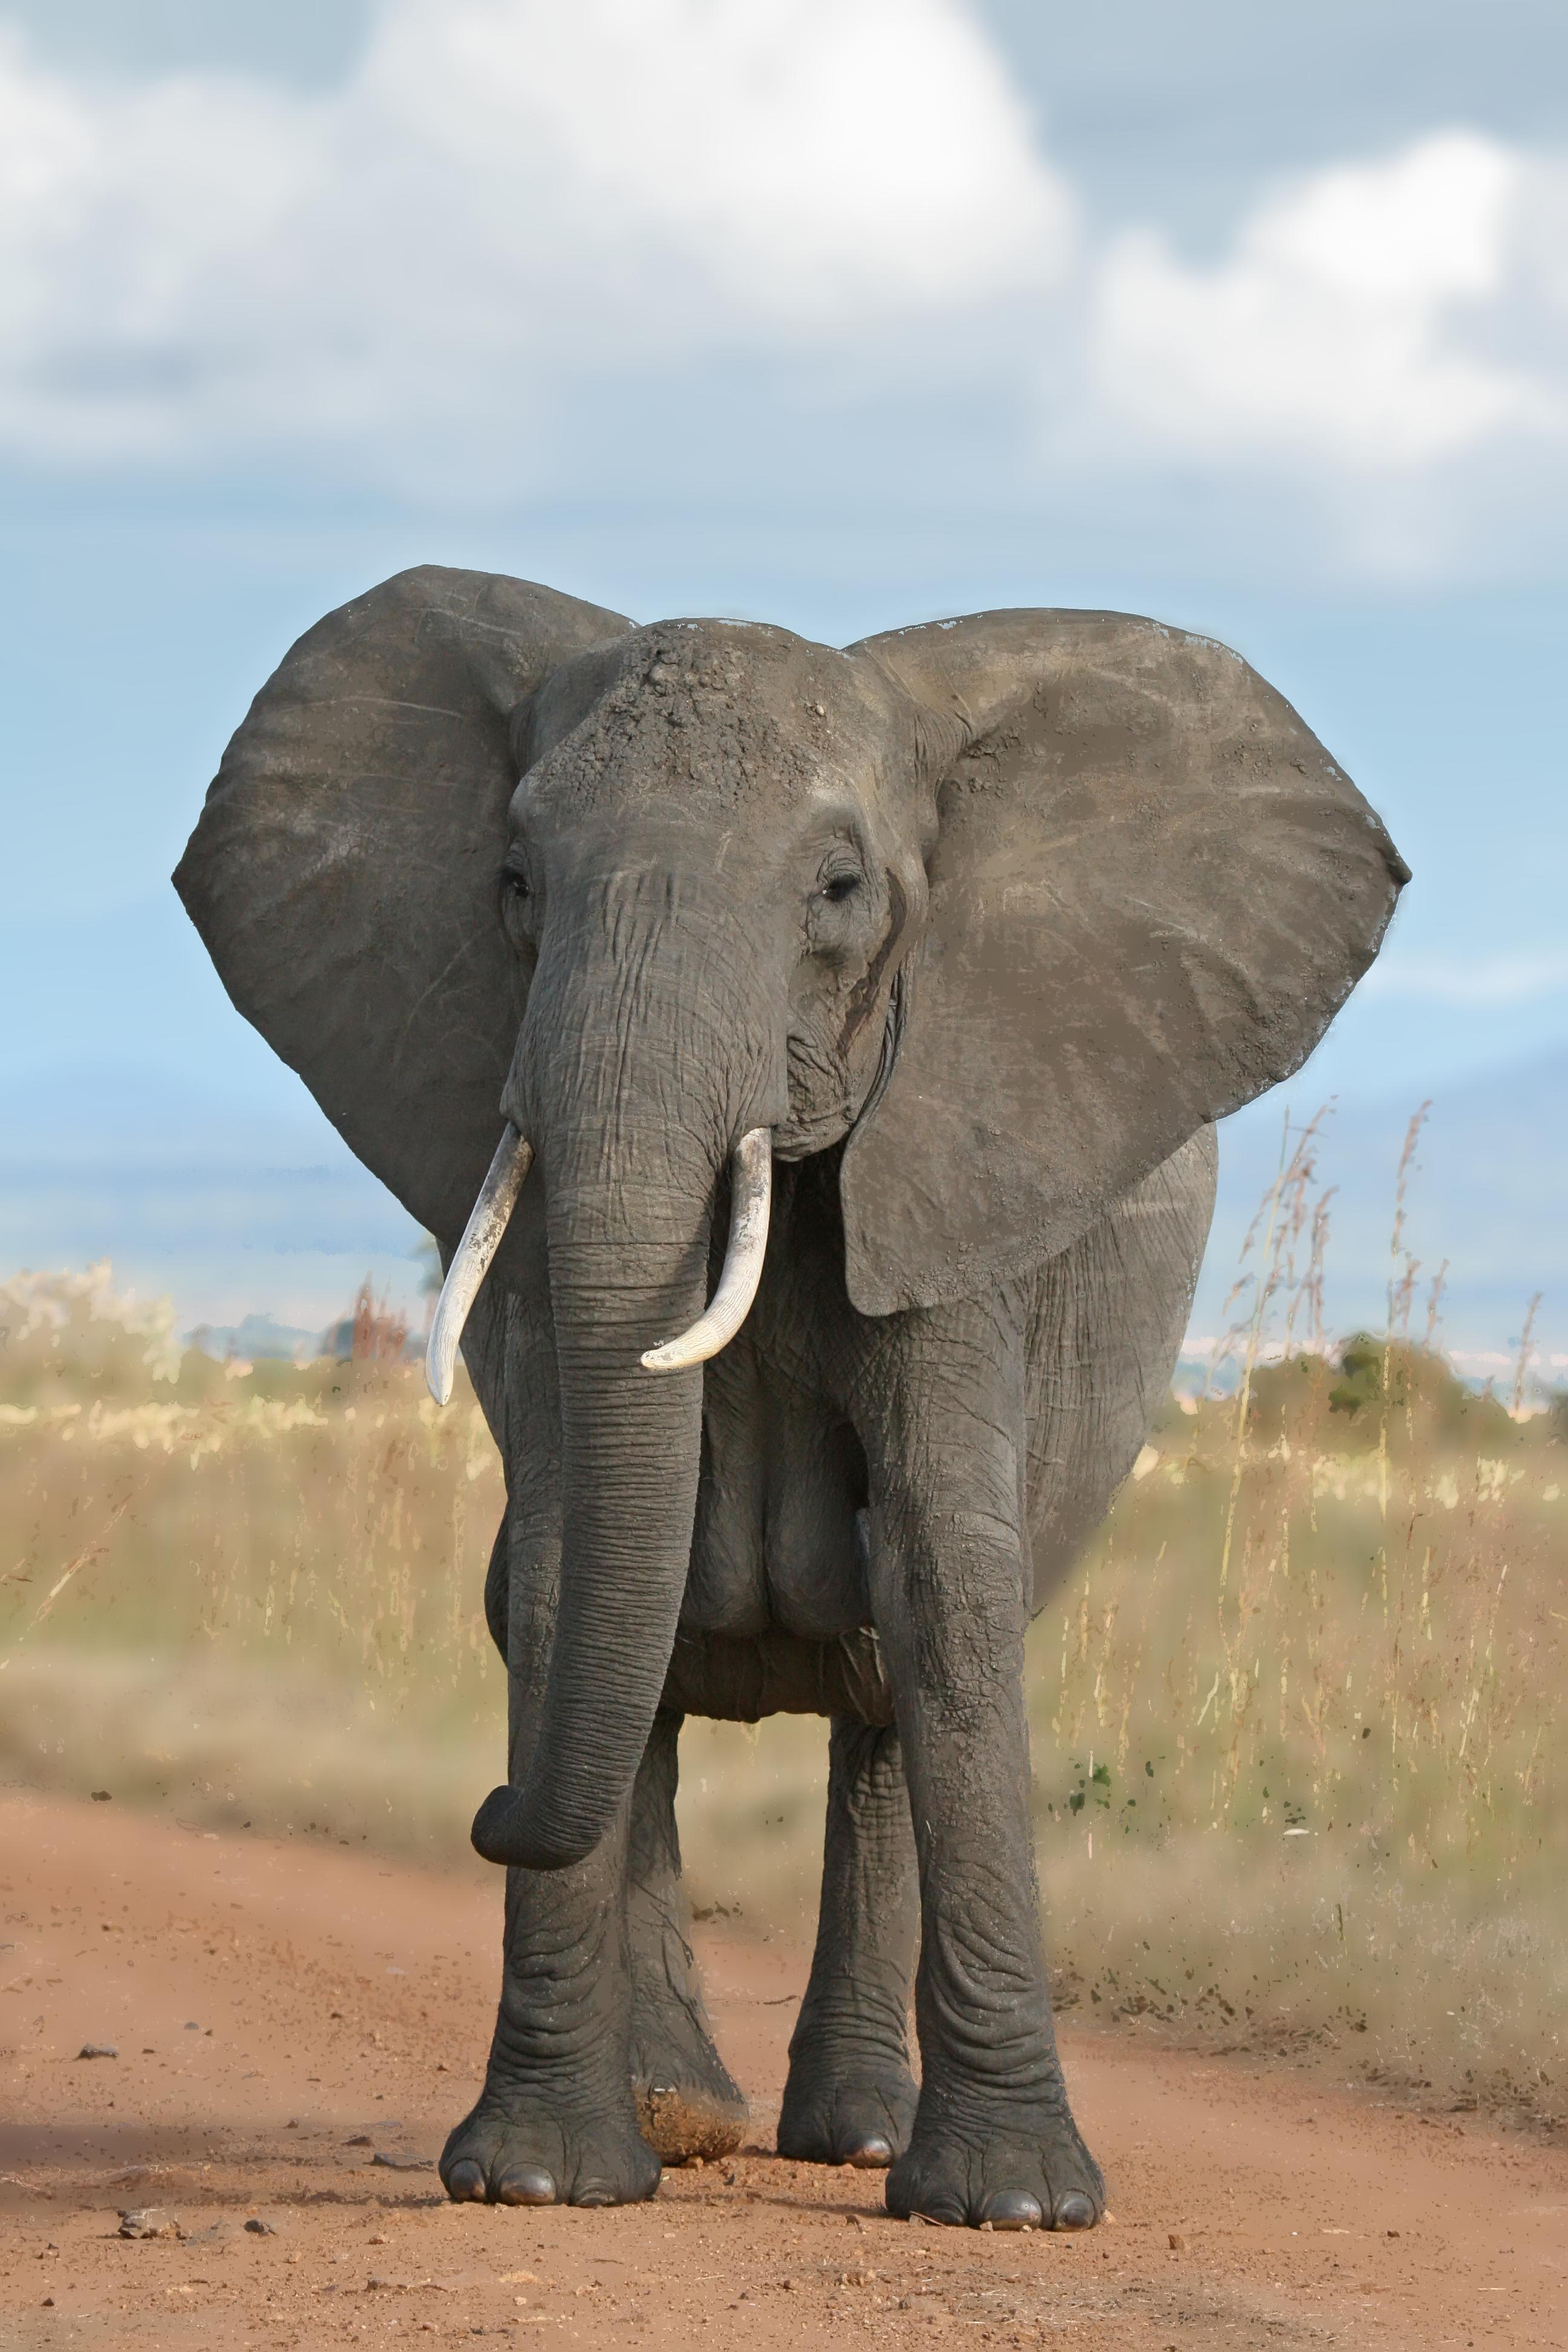
\includegraphics[width=0.9\linewidth]{large_elephant_portrait.jpg}
        \caption{Output Portrait Mode Image}
    \end{minipage}\hfill
\end{figure}

\section{Algorithm}

We used a simplified version of the grab-cut algorithm, with the idea of getting
the color distribution of the background to find the foreground.
Our algorithm takes in input image and returns the image in portrait mode.
Each image is represented as an array of pixels, with each pixel representing
a red, green, and blue value.

Each step of the algorithm will be referred to its shortened name in
parenthesis.
\begin{enumerate}
    \item
        Designiate the borders of the image as the background. Top, left, and
        right $\tfrac{1}{8}$ of image.
    \item
        Get a color distribution of the background region. Group colors together
        based on a certain threshold. (Color Counts)
    \item
        Create a foreground mask by finding every pixel with a color not
        in the background color distrubution. Filter colors that make up
        less than 1 percent of the background area. (Build Mask)
    \item
        For every unmasked pixel, add it to the mask if two of its neighboring
        pixels were part of the mask. (Refine Mask)
    \item
        Blur all the pixels that are not within the foreground mask. We used a
        convolution with a circular filter to emulate the bokeh effect. (Blur)
    \item
        For each pixel in the mask, add the original pixel of the image into
        the blurred version of the image.
\end{enumerate}

\begin{figure}[!htb]
    \begin{minipage}{0.48\textwidth}
        \centering
        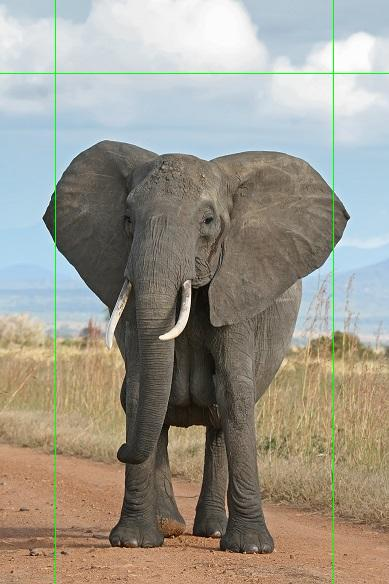
\includegraphics[width=0.5\linewidth]{border.jpg}
        \caption{Background Region (Step 1)}
    \end{minipage}\hfill
    \begin{minipage}{0.48\textwidth}
        \centering
        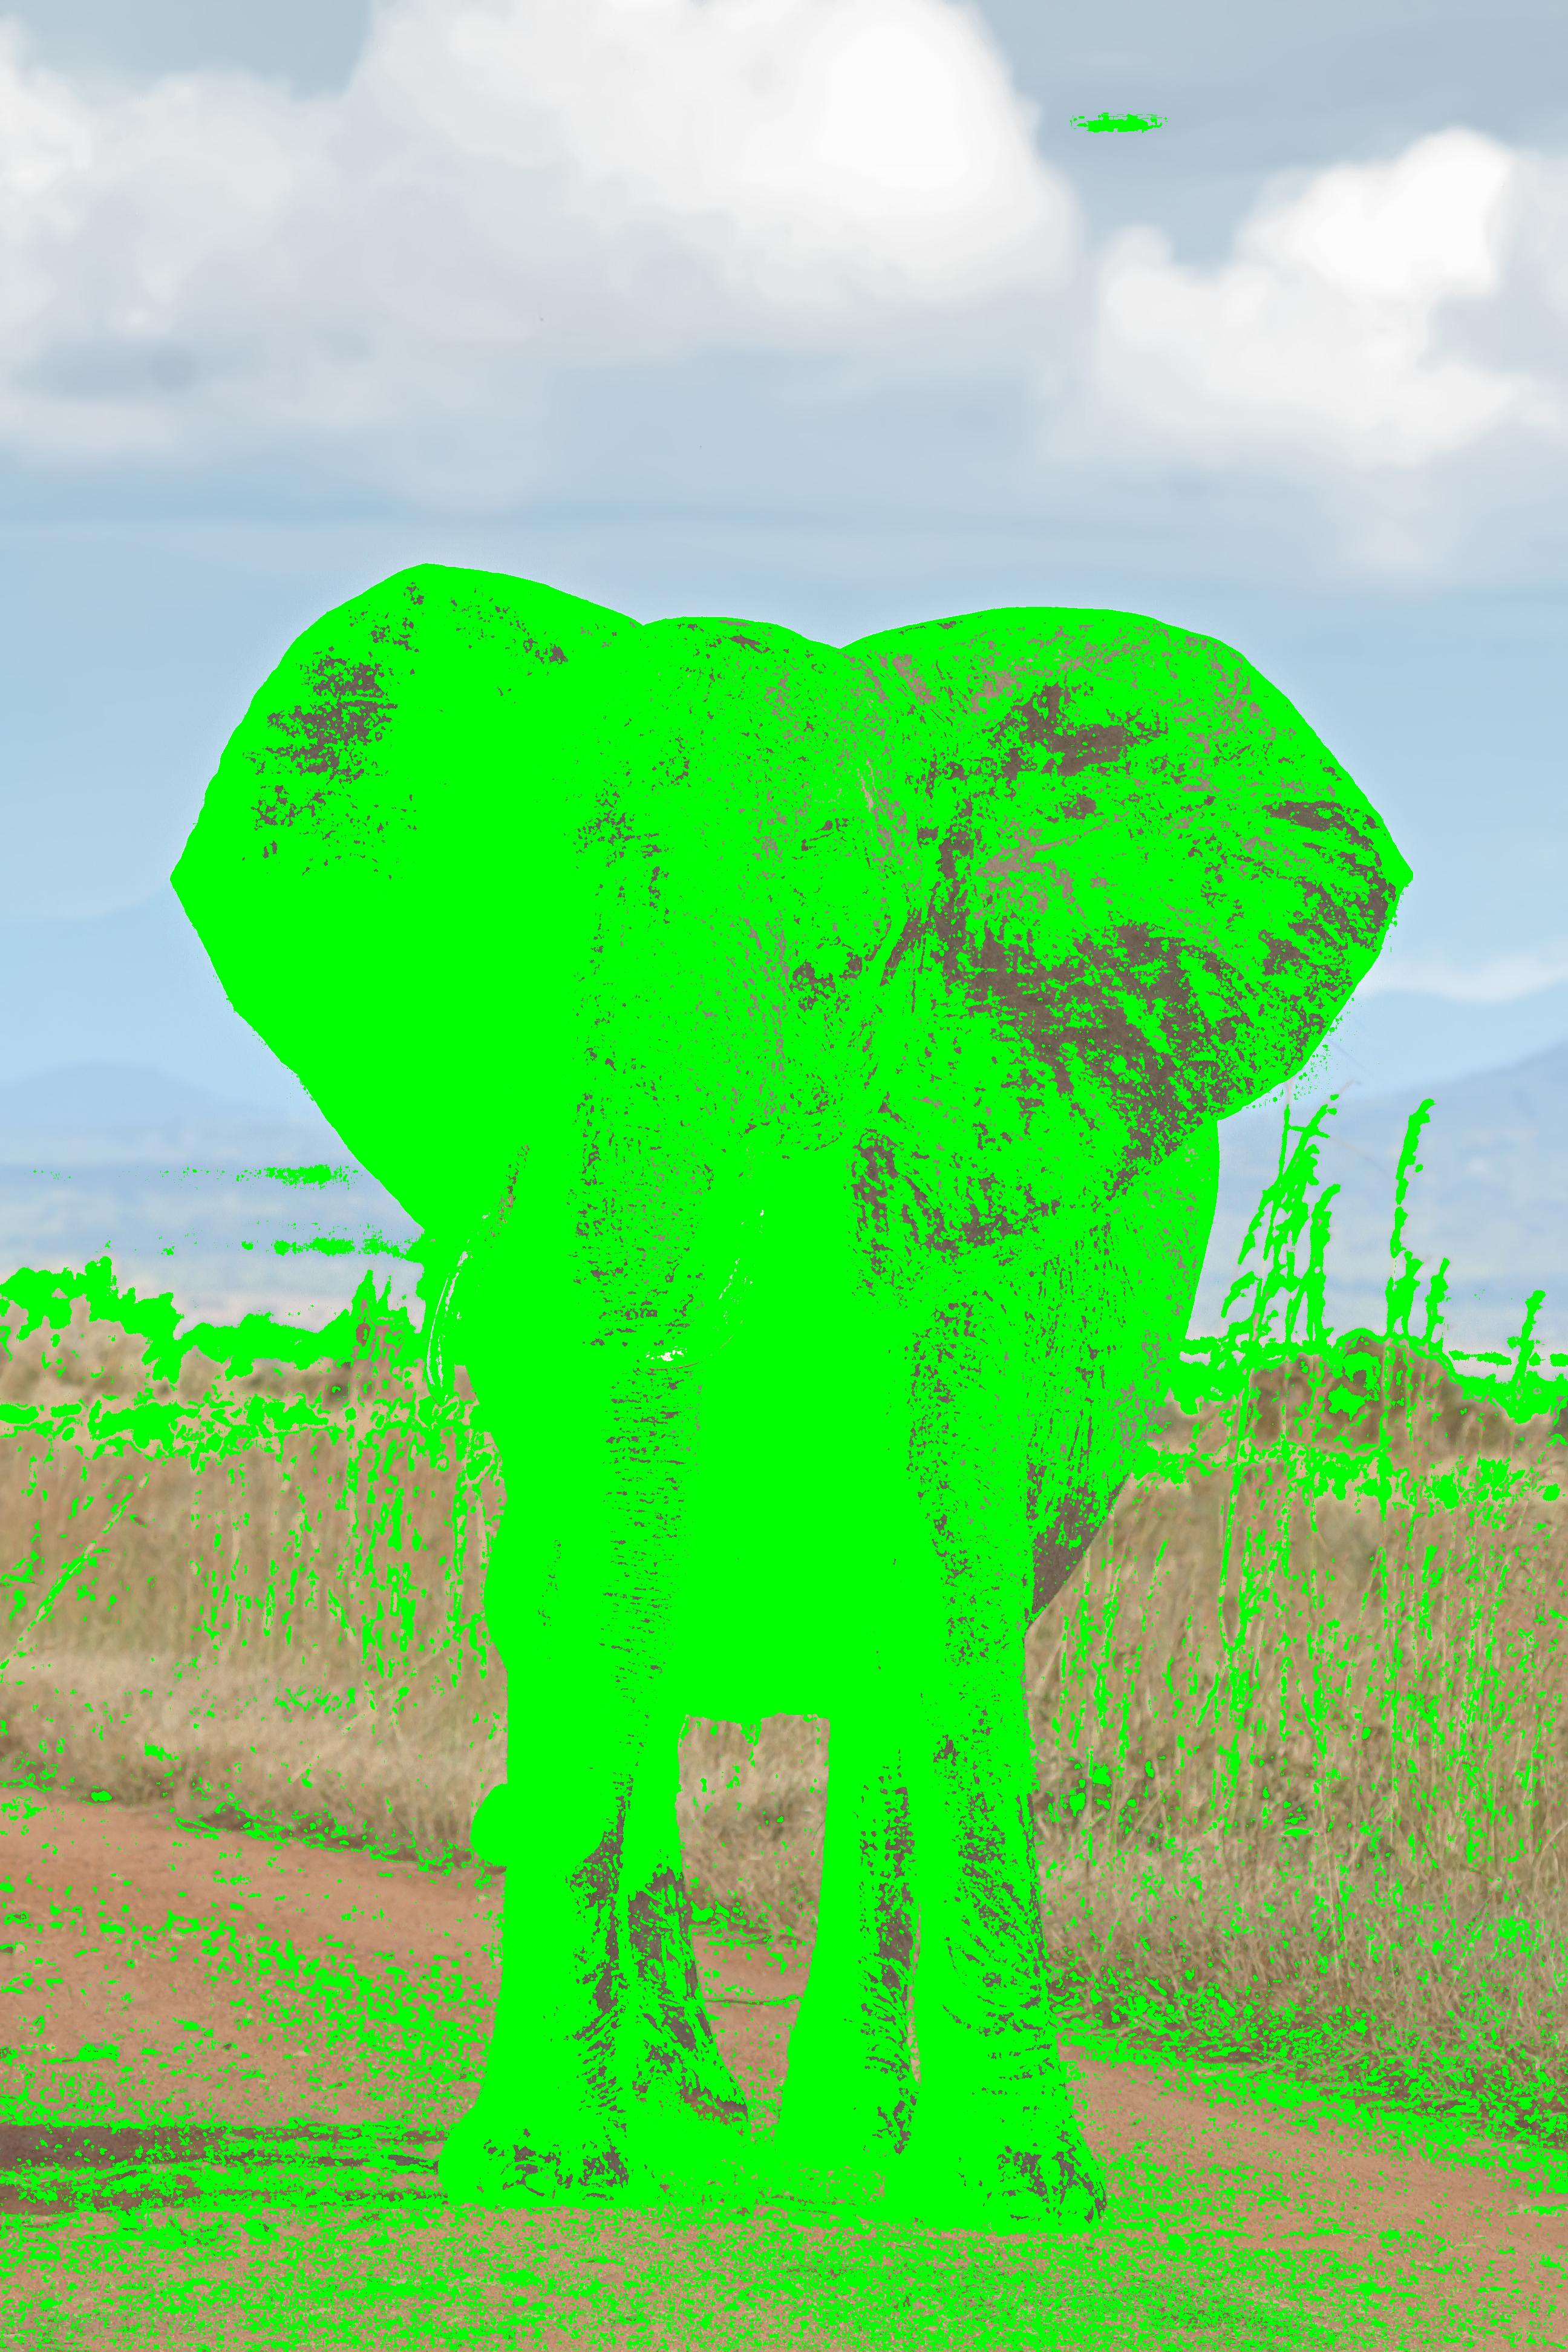
\includegraphics[width=0.5\linewidth]{mask.jpg}
        \caption{Foreground Mask (Step 5)}
    \end{minipage}\hfill
\end{figure}

\subsection{Data Structures}
We stored the color distribution by creating color buckets for every RGB value.
Essentially, all colors in one bucket would be within 15 red, green, and blue
value. This results in $\tfrac{255/15}^3$ different buckets.

\subsection{Background}
The blur is the most computationally intensive part of the algorithm. Each pixel
of the blurred image needs to compute the average RGB values for a circle
of pixels around it. However, the blur is data parallel, as each pixel is
independent.

However, each step of the algorithm has to be finished before the next step.
This requires synchronization after each step.

\section{Approach}
We were interested in comparing the GPU and CPU implementations of
our algorithm, so we implemented it in CUDA and OpenMP.
To develop and solidify our algorithm, we first wrote an implementation with
Python's NumPy before moving on to sequential C and then parallelism.

\section{CUDA on GPUS}
We utilized the NVIDIA 1080x GPUs in the Gates Clusters with CUDA.

\subsection{Color Counts}
Our color distribution

\subsection{Blur}
We were able to take advantage of the data parallelism for the blur, as each
pixel's computation was indepedent from those of other pixels. So, each pixel
is mapped to one CUDA thread. Additionally, pixels spatially close are mapped to
the same block. This allowed us to take advantage of the high
amount of threads in each SM. This mapping significantly decreased the
arithmetic computation per thread, but we realized that we had a memory
bottleneck.

We noticed that the pixels close together needed to access the same neighboring
pixels to perform the convolution. So, we loaded every pixel needed for that
block's blur into shared memory. The kernel that contained the weights for how
much each neighboring pixel contributed to the average was also loaded into
shared memory. By having each thread load data into shared
memory, the cost of loading it is very low while allowing every memory
access to be from shared memory.

\begin{center}
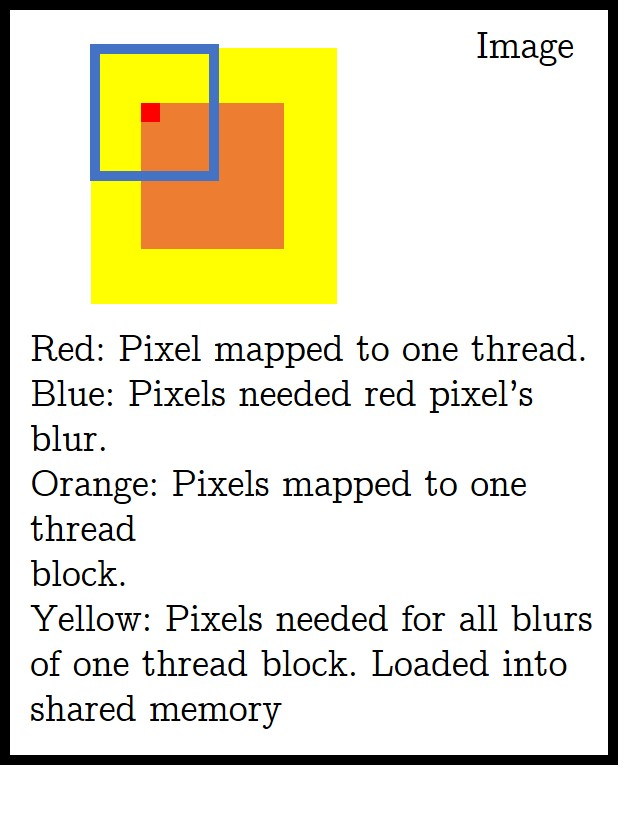
\includegraphics[scale=0.3]{mapping.jpg} \\
Thread mapping and shared memory
\end{center}

\section{Results}

\subsection{Bluejay}
\begin{tabular}{l|l|l|l|l|l}
    Item & C & OMP & Speedup & CUDA & Speedup
\\  \hline
    init & 0.00096 & 0.00129 & 0.74244 & 0.13345 & 0.00717
\\  color counts & 0.00167 & 0.00224 & 0.74365 & 0.00003 & 50.54545
\\  build mask & 0.00451 & 0.00473 & 0.95389 & 0.00031 & 14.50161
\\  refine mask & 0.00301 & 0.00446 & 0.67422 & 0.00001 & 250.58333
\\  blur & 11.72630 & 1.08236 & 10.83397 & 0.02218 & 528.56863
\\  clean up & 0.04040 & 0.05069 & 0.79694 & 0.04784 & 0.84449
\end{tabular}
\subsection{Elephant}
\begin{tabular}{l|l|l|l|l|l}
    Item & C & OMP & Speedup & CUDA & Speedup
\\  \hline
    init & 0.00036 & 0.00040 & 0.89873 & 0.15685 & 0.00226
\\  color counts & 0.00039 & 0.00029 & 1.34021 & 0.00004 & 10.26316
\\  build mask & 0.00113 & 0.00355 & 0.31748 & 0.00010 & 11.28000
\\  refine mask & 0.00069 & 0.00345 & 0.19977 & 0.00001 & 49.21429
\\  blur & 2.06310 & 0.19922 & 10.35614 & 0.00490 & 421.21254
\\  clean up & 0.01164 & 0.01255 & 0.92750 & 0.01214 & 0.95906
\end{tabular}
\subsection{Flower}
\begin{tabular}{l|l|l|l|l|l}
    Item & C & OMP & Speedup & CUDA & Speedup
\\  \hline
    init & 0.00439 & 0.00499 & 0.88127 & 0.15777 & 0.02785
\\  color counts & 0.01046 & 0.01043 & 1.00278 & 0.00004 & 261.45000
\\  build mask & 0.02424 & 0.00688 & 3.52537 & 0.00154 & 15.71225
\\  refine mask & 0.01356 & 0.00699 & 1.93991 & 0.00002 & 753.22222
\\  blur & 71.95433 & 6.17977 & 11.64353 & 0.10214 & 704.47463
\\  clean up & 0.23239 & 0.21021 & 1.10548 & 0.20083 & 1.15712
\end{tabular}
\subsection{Large Elephant}
\begin{tabular}{l|l|l|l|l|l}
    Item & C & OMP & Speedup & CUDA & Speedup
\\  \hline
    init & 0.01143 & 0.01031 & 1.10873 & 0.18277 & 0.06254
\\  color counts & 0.03089 & 0.01976 & 1.56346 & 0.00004 & 702.13636
\\  build mask & 0.06746 & 0.01338 & 5.04223 & 0.00269 & 25.09673
\\  refine mask & 0.03535 & 0.01292 & 2.73672 & 0.00002 & 1767.65000
\\  blur & 111.87493 & 9.92077 & 11.27684 & 0.17171 & 651.53039
\\  clean up & 0.42162 & 0.39693 & 1.06220 & 0.48704 & 0.86568
\end{tabular}
\subsection{Purp}
\begin{tabular}{l|l|l|l|l|l}
    Item & C & OMP & Speedup & CUDA & Speedup
\\  \hline
    init & 0.01087 & 0.00793 & 1.37112 & 0.14426 & 0.07537
\\  color counts & 0.03020 & 0.01008 & 2.99524 & 0.00004 & 774.30769
\\  build mask & 0.05580 & 0.00681 & 8.19369 & 0.00183 & 30.45797
\\  refine mask & 0.02416 & 0.00791 & 3.05347 & 0.00002 & 1342.00000
\\  blur & 88.81756 & 7.20338 & 12.32998 & 0.11458 & 775.17792
\\  clean up & 0.36895 & 0.32241 & 1.14435 & 0.29950 & 1.23189
\end{tabular}
\subsection{Tiger}
\begin{tabular}{l|l|l|l|l|l}
    Item & C & OMP & Speedup & CUDA & Speedup
\\  \hline
    init & 0.00164 & 0.00106 & 1.55052 & 0.13512 & 0.01215
\\  color counts & 0.00342 & 0.00168 & 2.04119 & 0.00003 & 106.84375
\\  build mask & 0.01004 & 0.00120 & 8.35554 & 0.00032 & 31.65615
\\  refine mask & 0.00698 & 0.00166 & 4.21679 & 0.00001 & 498.78571
\\  blur & 14.74396 & 1.30024 & 11.33942 & 0.02366 & 623.05451
\\  clean up & 0.06286 & 0.04768 & 1.31833 & 0.04895 & 1.28423
\end{tabular}

\end{document}
